\documentclass{report}
\usepackage[utf8]{inputenc}
\usepackage[T1]{fontenc}
\usepackage{CormorantGaramond}
\usepackage{fontspec}
\usepackage{geometry}
\usepackage[table]{xcolor}
\usepackage{tabularx}
\usepackage{graphicx}
\usepackage{mathtools}
\usepackage[bottom]{footmisc}
\usepackage[italian]{babel}
\usepackage{hyperref}
\usepackage{titlesec}
\usepackage{listings}
\usepackage{color}
\usepackage{graphicx}
\usepackage{xltabular}
\usepackage{fancyhdr}
\usepackage{pgf-pie}
\usepackage{float}

\renewcommand{\headrulewidth}{0.4pt}
\renewcommand{\footrulewidth}{0.4pt}

\lstset{ % General setup for the package
    basicstyle=\small\sffamily,
    numbers=left,
     numberstyle=\tiny,
    frame=tb,
    tabsize=4,
    columns=fixed,
    showstringspaces=false,
    showtabs=false,
    keepspaces,
    commentstyle=\color{red},
    keywordstyle=\color{blue}
}

\geometry{
a4paper,
total = {170mm, 240mm},
left = 20mm,
top = 20mm,
}

\setlength{\headheight}{33.60004pt}

\setlength{\parindent}{0em}
\setlength{\parskip}{0.7em}

\titlespacing{\section}{0pt}{0.7em}{0.5em}
\titlespacing{\subsection}{0pt}{0.7em}{0.5em}

\newcommand{\gassets}{../}

\renewcommand{\title}{
    Manuale utente
    
    \tiny Versione documento: \textit{V0.0.2}
}

\newcommand{\people}{
    \normalsize
    \begin{center}
        \begin{tabularx}{7cm}{l | X}            
            \textbf{Uso} & Esterno\\
            \textbf{Destinatario} & Committente\\
            & Cliente \\
        \end{tabularx}
    \end{center}
}

\fancypagestyle{plain}{%
    \fancyhead{} % clear all header fields
    \fancyhead[L]{\leftmark}
    \fancyhead[R]{\textit{SWEasabi} \includegraphics[height=30pt]{\gassets global-assets/img/loghi/SWEasabi_compact_logo.png}}
    \fancyfoot{} % clear all footer fields
    \fancyfoot[L]{\thepage}
    \fancyfoot[R]{Manuale utente}
}

\begin{document}

\pagestyle{fancy}

\fancyhead{} % clear all header fields
\fancyhead[L]{\leftmark}
\fancyhead[R]{\textit{SWEasabi} \includegraphics[height=30pt]{\gassets global-assets/img/loghi/SWEasabi_compact_logo.png}}
\fancyfoot{} % clear all footer fields
\fancyfoot[L]{\thepage}
\fancyfoot[R]{Manuale utente}


\input{\gassets global-assets/tex/header}
\thispagestyle{empty}
\clearpage
\pagenumbering{Roman}
\section*{Registro delle modifiche}

\newcommand{\pzerozerouno}{
    \begin{center}
        \begin{tabularx}{\linewidth}{l | X}
            \textbf{Approvazione} & Romano Davide\\
            \hline
            \textbf{Redazione}& Peron Samuel\\
            & Zarantonello Giorgio\\
            \hline
            \textbf{Verifica} & Pierobon Luca\\
            & Massarenti Alessandro\\
            & Bonavigo Michele \\
        \end{tabularx}
    \end{center}
}
\newcommand{\mzerozerouno}{
    \begin{itemize}
        \item Prima stesura del documento e definzione struttura
    \end{itemize}
}

\newcommand{\vzerozerouno}{
    \hline
    0.0.1 & 21 lug 2023 & \mzerozerouno & \pzerozerouno\\
}
\newcommand{\pzerozerodue}{
    \begin{center}
        \begin{tabularx}{\linewidth}{l | X}
            \textbf{Approvazione} & Romano Davide\\
            \hline
            \textbf{Redazione}& Peron Samuel\\
            & Zarantonello Giorgio\\
            \hline
            \textbf{Verifica} & Pierobon Luca\\
            & Massarenti Alessandro\\
            & Bonavigo Michele \\
        \end{tabularx}
    \end{center}
}
\newcommand{\mzerozerodue}{
    \begin{itemize}
        \item Miglioramento del documento
    \end{itemize}
}

\newcommand{\vzerozerodue}{
    \hline
    0.0.2 & 28 lug 2023 & \mzerozerodue & \pzerozerodue\\
}
\newcommand{\pzerounozero}{
    \begin{center}
        \begin{tabularx}{\linewidth}{l | X}
            \textbf{Verifica} & Pierobon Luca\\
        \end{tabularx}
    \end{center}
}
\newcommand{\mzerounozero}{
    \begin{itemize}
        \item Revisione del documento
    \end{itemize}
}

\newcommand{\vzerounozero}{
    \hline
    0.1.0 & 17 ago 2023 & \mzerounozero & \pzerounozero\\
}
\newcommand{\punozerozero}{
    \begin{center}
        \begin{tabularx}{\linewidth}{l | X}
            \textbf{Approvazione} & Romando Davide\\
        \end{tabularx}
    \end{center}
}
\newcommand{\munozerozero}{
    \begin{itemize}
        \item Approvazione del documento
    \end{itemize}
}

\newcommand{\vunozerozero}{
    \hline
    1.0.0 & 17 ago 2023 & \munozerozero & \punozerozero\\
}
%Tabella
\begin{center}
    \begin{xltabular}{\linewidth}{|l|l|X|X|}
        \hline
        \textbf{Versione} & \textbf{Data} & \textbf{Modifica}& \textbf{Persone}\\
        \vunozerozero
        \vzerounozero
        \vzerozerodue
        \vzerozerouno
        \hline
    \end{xltabular}
\end{center}

\tableofcontents
\clearpage
\pagenumbering{arabic}
\chapter{Scopo del documento}

Questo documento ha lo scopo di fornire una descrizione dettagliata del comportamento e delle specifiche per l'Utente Gestore e l'Utente Manutentore nel contesto del nostro progetto di Ingegneria del Software. Entrambi gli utenti svolgono ruoli chiave all'interno del sistema e dispongono di funzionalità specifiche per eseguire le loro attività.
\newline\newline
\textbf{L'Utente Gestore }è responsabile della gestione e del monitoraggio generale del sistema.
\newline\newline
\textbf{L'Utente Manutentore }si occupa della manutenzione del sistema, intervenendo per risolvere problemi e mantenere le entità in condizioni ottimali. 

\chapter{Utente Gestore}

\section{Cosa può fare l'Utente Gestore}
L'Utente Gestore ha il potere di svolgere diverse attività all'interno del sistema. Di seguito, vengono elencate le principali funzionalità:

\subsection{Aprire Ticket}
L'Utente Gestore ha la possibilità di aprire nuovi ticket. 
I ticket rappresentano richieste o problemi segnalati all'\textit{Utente Manutentore}.
Ogni ticket viene gestito da un entità esterna.

\subsection{Visualizzare Ticket}
L'Utente Gestore può visualizzare l'elenco dei ticket esistenti. 

\subsection{Visualizzare le Entità: Area, Lampada e Sensori}
Il Gestore ha la possibilità di visualizzare le diverse entità del sistema, tra cui:
\begin{itemize}
\item \textbf{Area}: Rappresenta una zona geografica gestita dall'applicazione, dove possono essere collocate una o più lampade e sensori. 
\item \textbf{Lampada}: Indica le fonti luminose nel sistema. Il Gestore può visualizzare informazioni sullo stato delle lampade ed il loro alias.
\item \textbf{Sensori}: Rappresentano i sensori collocati in diverse aree del progetto. Il Gestore può visualizzare le informazioni dei sensori come Alias, posizione geografica e portata.
\end{itemize}


\chapter{Utente Manutentore}

\section{Cosa può fare l'Utente Manutentore}
L'Utente Manutentore ha il potere di svolgere diverse attività all'interno del sistema. Di seguito, vengono elencate le principali funzionalità:

\subsection{Chiudere Ticket}
L'Utente Manutentore ha la possibilità di chiudere ticket. 
I ticket rappresentano richieste o problemi segnalati dall'\textit{Utente Gestore}.

\subsection{Visualizzare Ticket}
L'Utente Manutentore può visualizzare l'elenco dei ticket esistenti. 

\subsection{Inserimento/rimozione delle Entità: Area, Lampada e Sensori}
Il Manutentore ha la possibilità di modificare le diverse entità del sistema, tra cui:
\begin{itemize}
\item \textbf{Area}: Rappresenta una zona geografica gestita dall'applicazione, dove possono essere collocate una o più lampade e sensori. 
\item \textbf{Lampada}: Indica le fonti luminose nel sistema. Il Manutentore può visualizzare informazioni sullo stato delle lampade ed il loro alias.
\item \textbf{Sensori}: Rappresentano i sensori collocati in diverse aree del progetto. Il Manutentore può visualizzare le informazioni dei sensori come Alias, posizione geografica e portata.
\end{itemize}
\chapter{Overview della webapp}

\section{Pagine webapp}

Dopo aver eseguito il login, l'utente viene reindirizzato alla pagina \textit{Dashboard lampioni} che fungera da pagina principale della webapp. Utilizzando i bottoni presenti nell'header della pagina sarà possibile spostarsi tra le varie pagine disponibili.

\section{Dashboard Lampioni}

Pagina in cui si viene automaticamente reindirizzati una volta eseguito il login, è inoltre possibile accedere a questa pagina premendo il relativo pulsante nell'header della pagina. In questa pagina vengono mostrati tutti i lampioni presenti a sistema e le loro informazioni, è inoltre possibile impostare una luminosità specifica su ognuno di essi, per applicare le modifiche basterà premere il pulsante conferma relativo al lampione desiderato \ref{fig:lista_lampioni}.

\begin{figure}[ht]
    \centering
    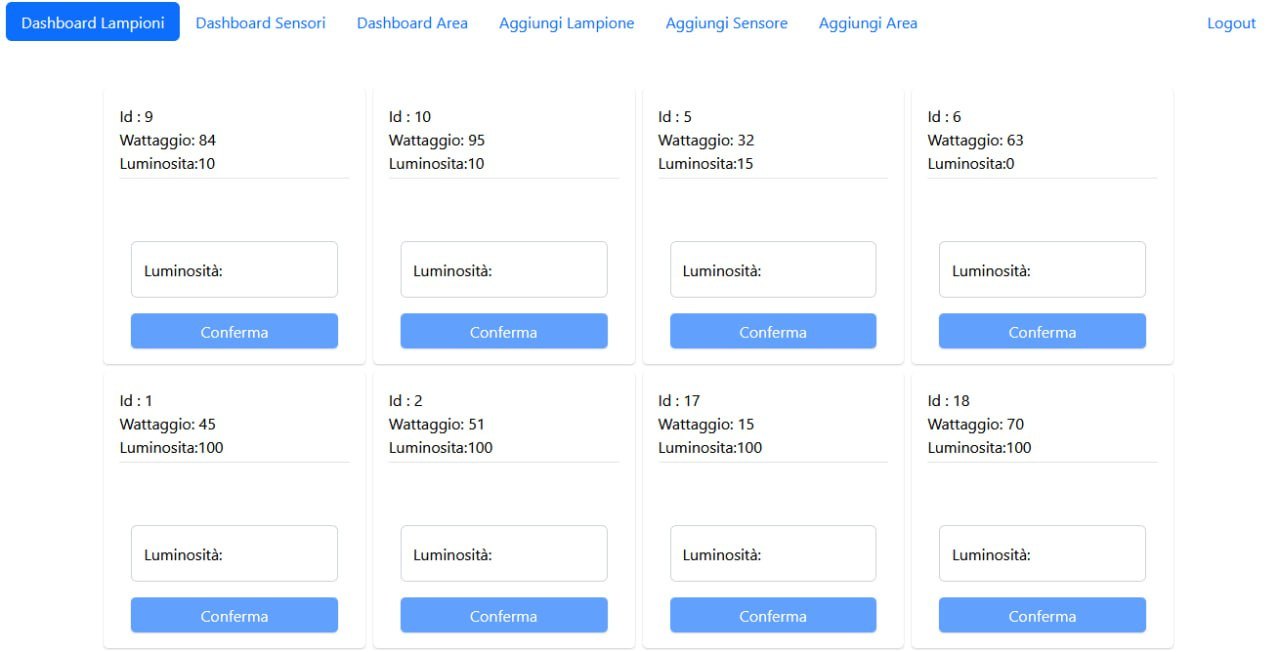
\includegraphics[width=\textwidth]{img/lista_lampioni.jpeg}
    \caption{Immagine della pagina Dashboard Lampioni.}
    \label{fig:lista_lampioni}
\end{figure}

\section{Dashboard Sensori}

Per accedere a questa pagina bisogna premere il relativo pulsante nell'header della pagina. In questa pagina vengono mostrati tutti i sensori presenti a sistema e le loro relative informazioni \ref{fig:lista_sensori}.

\begin{figure}[ht]
    \centering
    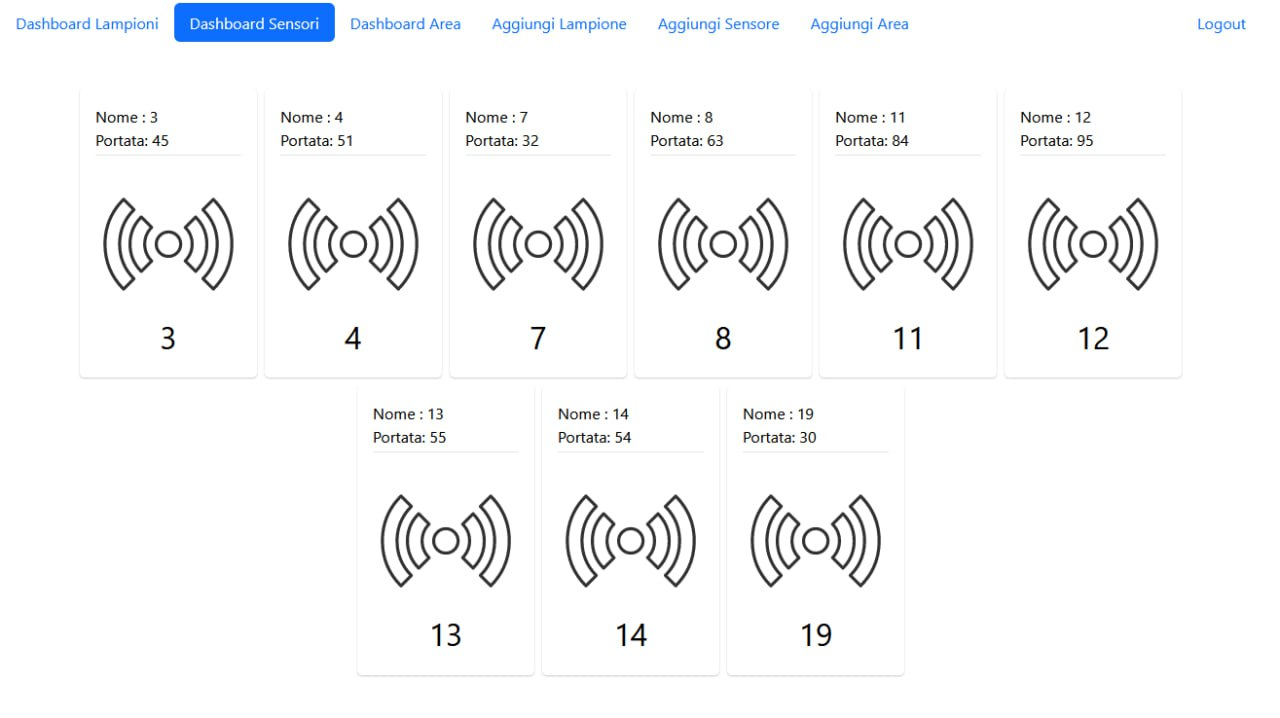
\includegraphics[width=\textwidth]{img/lista_sensori.jpeg}
    \caption{Immagine della pagina Dashboard Sensori.}
    \label{fig:lista_sensori}
\end{figure}

\section{Dashboard Area}

Per accedere a questa pagina bisogna premere il relativo pulsante nell'header della pagina. In questa pagina vengono mostrati tutte le areee presenti a sistema e le loro relative informazioni \ref{fig:lista_area}.

\begin{figure}[ht]
    \centering
    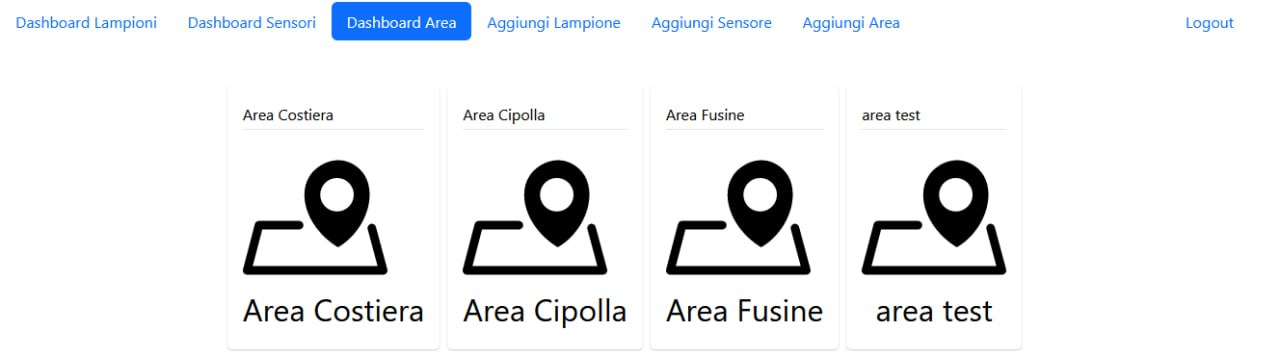
\includegraphics[width=\textwidth]{img/lista_area.jpeg}
    \caption{Immagine della pagina Dashboard Area.}
    \label{fig:lista_area}
\end{figure}

\section{Aggiungi Lampione}

Per accedere a questa pagina bisogna premere il relativo pulsante nell'header della pagina. In questa pagina è presente un form che permette di aggiungere un lampione a sistema digitando nei relativi campi le informazioni relative al lampione(idArea,latitudine,longitudine e wattaggio) e premendo il pulsante conferma per effettuare l'aggiunta a sistema del lampione desiderato \ref{fig:aggiunta_lamp}.

\begin{figure}[ht]
    \centering
    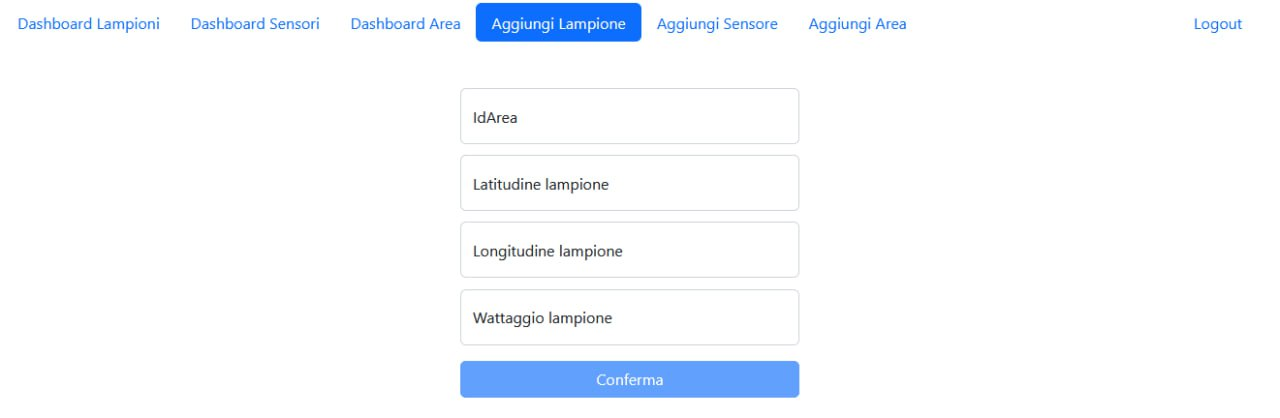
\includegraphics[width=\textwidth]{img/aggiunta_lamp.jpeg}
    \caption{Immagine della pagina Aggiungi Lampioni.}
    \label{fig:aggiunta_lamp}
\end{figure}

\section{Aggiungi Sensore}

Per accedere a questa pagina bisogna premere il relativo pulsante nell'header della pagina. In questa pagina è presente un form che permette di aggiungere un sensore a sistema digitando nei relativi campi le informazioni relative al sensore(idArea,latitudine,longitudine e raggio) e premendo il pulsante conferma per effettuare l'aggiunta a sistema del sensore desiderato \ref{fig:aggiunta_sens}.

\begin{figure}[ht]
    \centering
    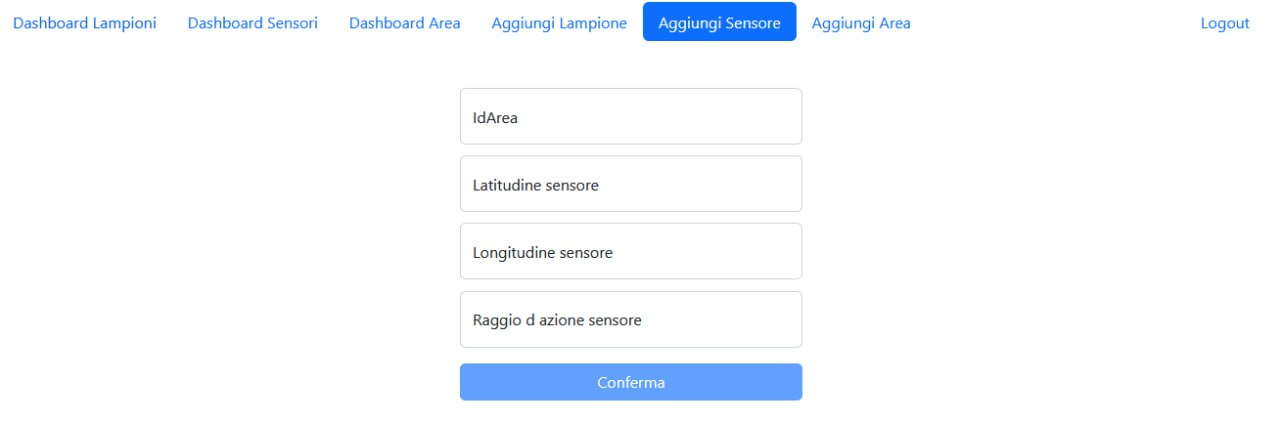
\includegraphics[width=\textwidth]{img/aggiunta_sens.jpeg}
    \caption{Immagine della pagina Aggiungi Sensori.}
    \label{fig:aggiunta_sens}
\end{figure}

\section{Aggiungi Area}

Per accedere a questa pagina bisogna premere il relativo pulsante nell'header della pagina. In questa pagina è presente un form che permette di aggiungere un' area a sistema digitando nei relativi campi le informazioni relative all'area(Alias) e premendo il pulsante conferma per effettuare l'aggiunta a sistema dell'area desiderata \ref{fig:aggiunta_area}.

\begin{figure}[ht]
    \centering
    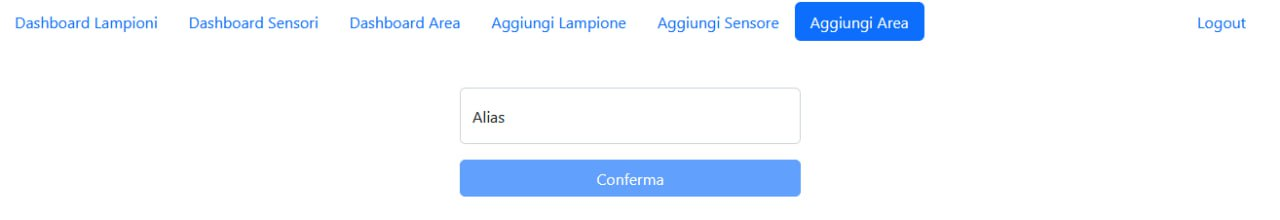
\includegraphics[width=\textwidth]{img/aggiunta_area.jpeg}
    \caption{Immagine della pagina Aggiungi Area.}
    \label{fig:aggiunta_area}
\end{figure}

\section{Logout}

Per disconnettersi dal proprio account basterà premere il pulsante \textit{Logout} presente nell'header della pagina.
\end{document}